Языки с зависимыми тпами обычно определяются через правила вывода (тут можно дать ссылочки на примеры, скажем на Мартин-Лёфа). Приводишь пример с Bool. (Сможешь написать его через правила вывода? Тебе нужно написать правила для переменных, правило, которое в тапл называлось T-Conv, и правила для Bool: Bool, true, false, if, редукции) Потом говоришь, что в нашей формализации по сути нужно вбить эти же правила, кроме первых двух, так как они являются общими для всех языков. Кроме того, иногда явно выписывают правила для отношения эквивалентности на термах, но у нас они тоже неявно подразумеваются. Потом показываешь как вводить эти правила на нашем языке, поясняешь, что означает то или иное обозначение. Отмечаешь какие есть отличия


Вдохновением данной работы послужила статьи~\cite{Palmgren} и~\cite{isaev}. Поэтому сам язык спецификации выглядит как язык описания алгебраических теорий\footnote{Алгебраическая теория это \textit{сигнатура} --- множество сортов и функциональных символов над ними --- и набор аксиом --- множество уравнений над термами, построенными с помощью типизированных переменных и функциональных символов. Сами функциональные символы тотальны, то есть применимы ко всем представителям данных сортов}.

А именно, помимо правил вывода у нас есть сорта и функциональные символы. Каждая конструкция в языке --- это функциональный символ в логике, а правила вывода и редукции --- это аксиомы. Правила вывода говорят, когда некоторый функциональный символ определен. Все функциональные символы являются частичными функциями, поэтому это существенно алгебраические теории, а не просто алгебраические. Частичные потому, что например конструкция if-then-else в качестве первого аргумента принимает только терм типа Bool, иначе она не определена и проверка типов должна уведомлять пользователя о некорректности сформированного терма.

Начнем с примера описания языка с зависимыми типами~(рис.\ref{lpi})~\cite[Глава~2.1]{book:pierce}

\begin{figure}
    \centering
	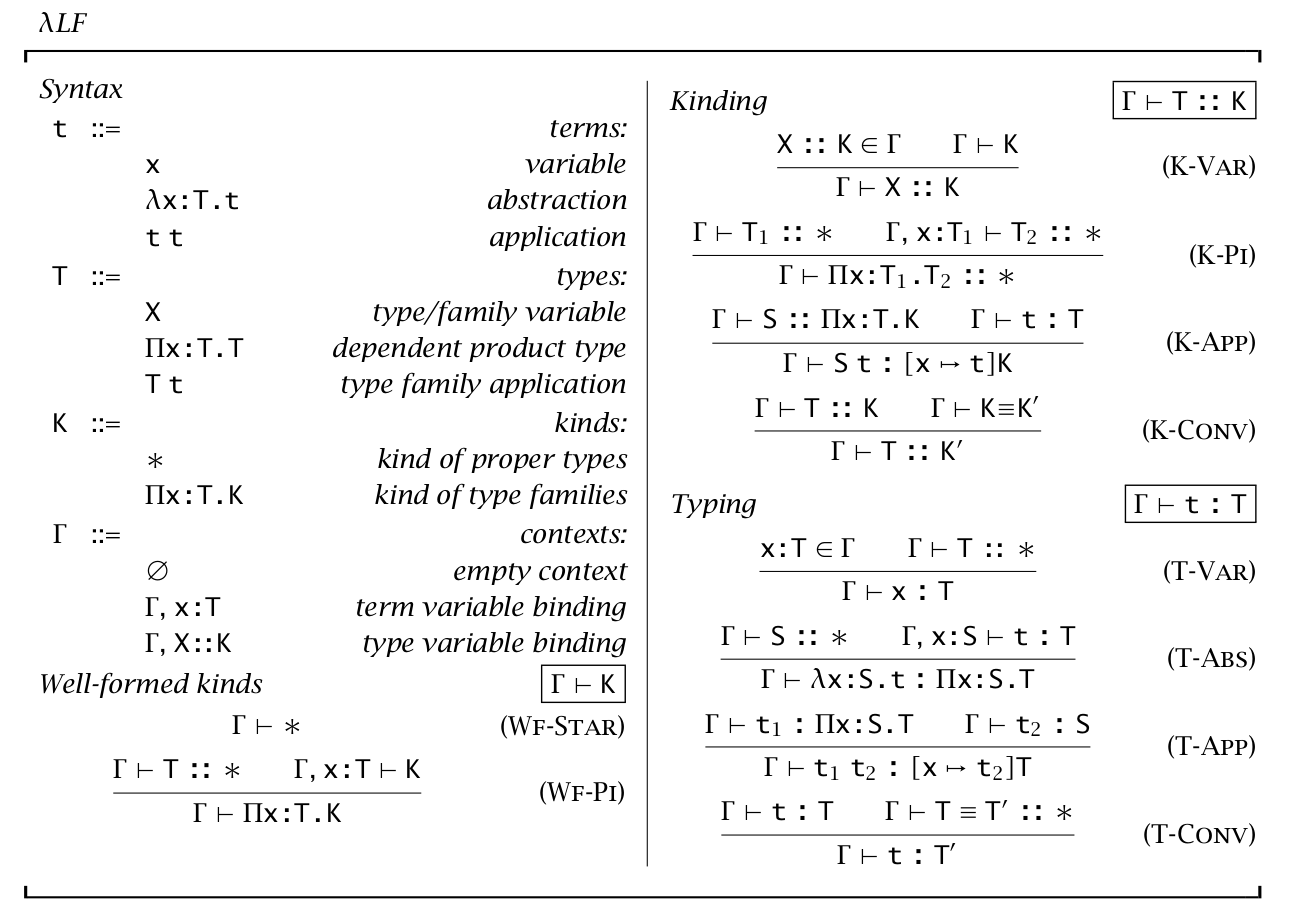
\includegraphics[scale=0.35]{img/lp.png}
	\caption{Язык с лямбдой и $\Pi$-типами }
	\label{lpi}
\end{figure}

В этом языке явно выделяются три сорта (можно думать о сортах как о метатипах): виды, термы и типы (правила связанные с видами и само их описание опущены для простоты).

Также явно выделяются примитивы языка (в дальнейшем мы называем их функциональными символами):
абстракция, $\Pi$-типы (функции в языках с зависимыми типами) и аппликация. Легко заметить, что во всех яхыках присутствуют подстановка, контексты, символ `:' означающий, что тип терма слева есть терм справа, и связывание переменных.

Правила вида T-Conv и T-Var всегда верны в зависимых языках, поэтому у нас они есть по умолчанию. Также подразумевается рефлексивность, симметричность, транзитивность и конгруэнтность равенства.

Если принять во внимания все наблюдения выше, то так этот язык будет выглядеть в нашем языке спецификации\footnote{Важно понимать, что запись $\_ \vdash$ не означает, что контекст пуст, если слева ничего не написано, это эквивалентно записи $\Gamma \vdash$.}:

\begin{lstlisting}[frame=single]
DependentSorts:
  tm, ty
FunctionalSymbols:
  lam: (ty, 0)*(tm, 1) -> tm
  app: (tm, 0)*(tm, 0)*(ty, 1) -> tm
  pi : (ty, 0)*(ty, 1) -> ty
Axioms:
  K-Pi =
    forall T1 : ty, x.T2 : ty
      x : T1 |- T2 def |--- |- pi(T1, x.T2) def
  TAbs =
    forall S : ty, x.T : ty, x.t : tm
      x : S |- t : T |--- |- lam(S, x.t) : pi(S, x.T)
  TApp =
    forall t1 : tm, t2 : tm, S : ty, x.T : ty
            |- t1 : pi(S, x.T),
            |- t2 : S,
      x : S |- T def
      |--------------------------
      |- app(t1, t2, x.T) : T[x:=t2]
Reductions:
  Beta =
    forall x.b : tm, A : ty, a : tm, z.T : ty
       |--- |- app(lam(A, x.b), a, z.T) => b[x:=a] : T[z:=a]
\end{lstlisting}

Типизирование метапеременных позволяет проверять правильность применения функциональных символов и наличие нужных переменных в контексте. Именованные переменные служат для определения порядка переменных в контексте и не несут какой-то дополнительной информации.

Также в язык была добавлена проверка на c-стабильность --- можно помечать аксиомы типами, тогда аксиома применима, только если все переменные входящие в терм являются представителями этих типов. Если список типов пуст, то производится проверка терма на отсутствие свободных переменных.
